\chapter{Projects}
\glsresetall

\section{Reinforcement Learning Research Paper}
\label{sec:research-paper}

At the start of my placement, my first project was to contribute to a research paper the company had
been working on. The subject of the paper revolved around \acro{ml}, \acrodesc{ml}.

As the company has a heavy focus on robotics, the paper focuses specifically on the application of
\acro{rl} on robotics. It is \acrodesc{rl}. As explained in \textcite{sutton2018reinforcement}, this
differs from other \acro{ml} approaches which focus on labelling unseen data based on previous
examples (Supervised Learning), or inferring structure and relations from unlabelled data
(Unsupervised Learning). In robotics, \acro{rl} is preferred over other \acro{ml} methods as it
allows for robots to learn and adapt complex behaviours from unstructured environments via the
\enquote{trial and error} method, without having to provide examples of the numerous complex
environments they could be deployed in.

Robotic environments commonly handle non-Euclidean data -- \glsdesc*{noneuclidean} -- for attributes
like orientations and stiffness. However, common reinforcement learning methods work under the
premise of Euclidean data -- \glsdesc*{euclidean} -- being used. This mismatch of data types lead to
non-Euclidean data being approximated under most contemporary methods. The paper's contribution
demonstrates a method to mitigate against this, by exploiting a specific non-Euclidean mathematical
construct (Riemannian geometry) in a way where data of non-Euclidean nature is preserved during
reinforcement learning training. Adapting these methods to be \enquote{geometry aware} can be shown
to increase accuracy during training, resulting in better policies (solutions) when applying
reinforcement learning.

\subsection{Training}

My specific role was to implement the theory of the paper in Python, run several experiments under
different environments comparing different approaches, generate accompanying visualizations, and
present my findings in the paper. As expected, this required extensive learning prior to me starting
my work. This came in the form of an online course provided by Coursera, which covered the
fundamentals of \acro{rl} from the works of \textcite{sutton2018reinforcement}. This was followed up
with an introduction to Deep RL -- reinforcement learning via neural networks -- by
\textcite{openai2018spinningup}.

Throughout my training, I gave presentations on these fundamental concepts and algorithms to other
colleagues, allowing me to receive valuable feedback in the areas I lacked clear explanations in and
helping me to evaluate gaps in my knowledge. My participation in the paper began when I had clearly
understood the fundamental premise of the paper along with some necessary background
knowledge.

This crash course in \acro{rl} was fairly enlightening, not only in academic knowledge, but also in
the effort it took to convey the knowledge in an accessible and understandable manner. Neither
presentation work nor essay writing were frequently exercised during my degree, and was therefore a
skill I had not exercised in a while. This would end up being a common theme during this project, as
the nature of a research paper is inherently to convey information in a manner which others can
understand.

\subsection{Research and experimentation}

Implementing the paper's proposed framework (Fig.~\ref{fig:paper-framework}) involved the
use of many technologies I had little experience with before. \gls*{pytorch}, \glsdesc*{pytorch},
was used in conjunction with \gls*{stablebaselines}, \glsdesc*{stablebaselines}, to reflect the
paper's proposal. I ran several experiments under simulation using the Gym Python library,
\glsdesc*{gympython}, to evaluate the paper's approach against several contemporary \acro{ml}
algorithms and other experimental approaches, including other related papers.

\begin{figure}
    \centering
    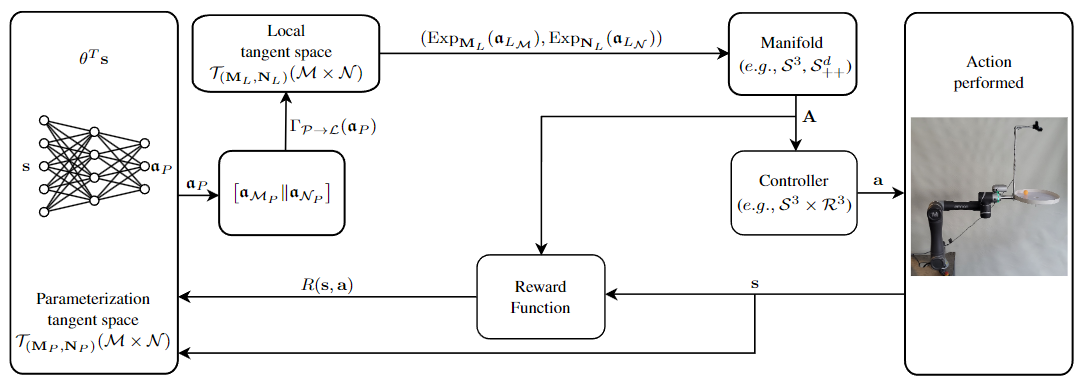
\includegraphics[width=\textwidth]{paper-pipeline}
    \caption{An illustration I created providing an overview of the proposed framework. The basic
        concept is transforming the output of a neural network in a way where Euclidean and
        non-Euclidean data are handled differently prior to being used.\label{fig:paper-framework}}
\end{figure}

This was a moderately challenging task, with many issues arising that I had not anticipated.
Ensuring my implementation of the paper was mathematically valid was critical, and many weeks were
spent with my manager and other researchers on the paper to ensure this was the case. This involved
the usage of both black-box and white-box testing, with my code validated against Matlab code
written by the researchers as a proof-of-concept. As my confidence in knowledge built up, I
challenged colleagues on some aspects of the code I found confusing or questionable, and had
constructive conversations on the best way to implement certain aspects of the proposed approach.

Additionally, the speed of execution was fairly slow due to the heavy use of neural networks being
computationally restricted by hardware limitations. Deep \acro{rl} significantly benefits from
strong GPUs due to the vast amount of computation neural networks require, with faster GPUs being
able to better utilise parallel processing at a larger scale. To work around this limitation, I made
use of Google's Colaboratory service, specifically designed for neural network and ML research which
provides access to data centre GPU computation. This resulted in a considerable performance
increase; what once took a weekend to process was now able to be completed in a matter of hours.

The results of the experiments were presented using \gls*{matplotlib}, \glsdesc*{matplotlib}, with
accompanying graphics created in \gls*{inkscape}, \glsdesc*{inkscape}, as seen in
Fig.~\ref{fig:paper-figures}. These were inserted alongside the text of the paper, which was typeset
with \LaTeX.

\begin{figure}
    \centering
    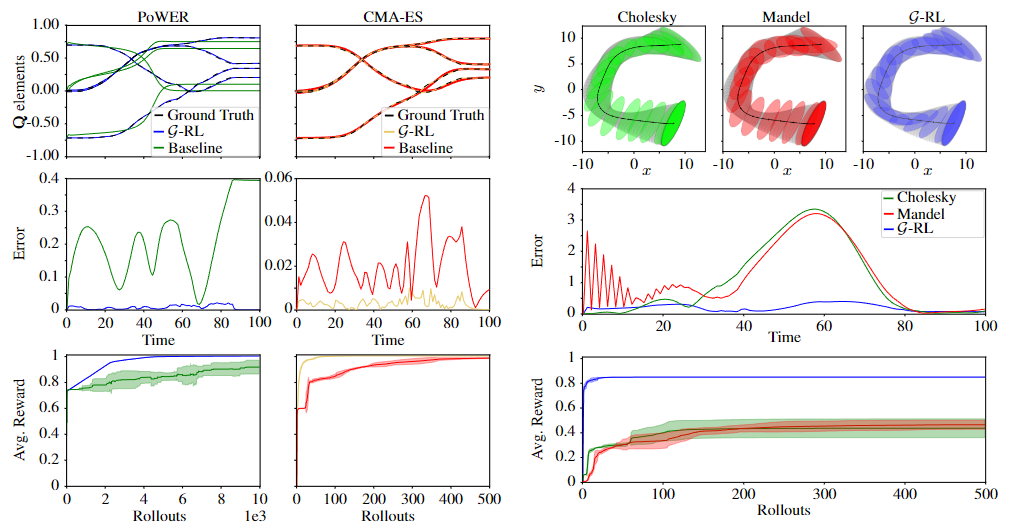
\includegraphics[width=\textwidth]{paper-results}
    \caption{A collection of graphs I created from experiment results.\label{fig:paper-figures}}
\end{figure}

An issue arose when collecting results as they had to be compiled from both Python and Matlab
codebases, across several machines (local and cloud-based). As Python and Matlab were saving results
in different data formats, I had to parse both into a common format which could then be read by
Pandas, \glsdesc*{pandaspython}. From this common format, I made use of Jupyter notebooks to
visualize and refine the resultant graphs to ensure they were clear to understand.

Although a straightforward problem to solve, this issue could have been completely avoided had some
more thought been put into how results would be collected, as everyone was focused on the
implementation of the experiments rather than the output format. A common generic format such as
\texttt{.csv} would have made collecting and visualising the data significantly easier.

When receiving feedback on the graphs I had generated, I discovered that my manager was colour-blind
and struggled to distinguish between data on the graph. Taking accessibility into account was not
something I had planned for, which I swiftly rectified with colour-blind friendly colours.
Responsibility lay on me to explain and evaluate the results of the experiments in the paper. This
again fell back to my knowledge gained during this project and conveying it in a clear manner, while
also following editorial guidelines of the publisher. The content, along with the rest of the paper,
was reviewed by all authors of the paper before being sent for review. As of the time of writing,
the paper has passed peer review and pending journal publication, available under
\textcite{alhousani2023geometric}

This project allowed me to throw myself into the deep end of \acro{ml}, using libraries and
algorithms I had not used before. While very challenging, the problem-solving process was very
enjoyable and piqued my interest in a new area of computer science. It also provided an insight into
academia I had not experienced before, causing me to consider pursuing academia related work in the
future.

\section{Robot Manipulation Library}
\label{sec:robot-library}

As the company was moving towards in-house software solutions for robotic software control, I was
tasked to assist in developing a C++ manipulation library using the
\acro{ros}\footnote{Counter-intuitively, \acro{ros} is \emph{not} an operating system in the
    traditional sense.}, \acrodesc{ros}, and \gls*{tesseract}, \glsdesc*{tesseract}.

The purpose of the task was to assess whether \gls*{tesseract} could be a viable alternative
compared to another popular planning framework, MoveIt. In comparison to MoveIt which is heavily
dependent on \acro{ros}, \gls*{tesseract} was \enquote{designed to be light-weight, limiting the
    number of dependencies, mainly only using standard [C++] libraries} \autocite{tesseractgithub}. If
possible to migrate to \gls*{tesseract}, the tight coupling and dependencies on \acro{ros} can be
significantly reduced. \gls*{tesseract} also holds other advantages over MoveIt, boasting the
ability to support dynamic reconfigurations of robots at runtime.

The details of the task involved the creation of a library that could execute motion using
waypoints, and motion via real-time teleoperation, working in both Cartesian space
(specifying a robot's end-effector in 3D coordinates) and joint space (specifying all of a robot's
joint orientations). The library also considered appropriately stopping motion when a joint limit is
reached, while being adaptable to any generic robot arm.

\subsection{Training}

To become comfortable programming with \acro{ros}, I worked on understanding the C++ tooling I would
be using (including build tools such as CMake and \acro{ros}-specific tools like \texttt{catkin}) as
well as going through several tutorials focusing on communication with simulated robots via
different methods, such as request-response and unidirectional observation data flows. I also tested
the trajectory controller (middleware to issue commands to robots) that I would end up using with
the library. The trajectory controller exposes a goal endpoint that accepts a trajectory
of joint positions across time. Once a goal is forwarded to the robot, the controller returns
several feedback states that correspond to the current progress of the action execution,
completing the action with a result state that indicates success or error.

Work on combining \gls*{tesseract} and \acro{ros} began once I felt confident building on top of
\acro{ros}. One major hurdle with \gls*{tesseract} is the notable lack of up-to-date documentation,
from installation to implementation, resulting in sometimes crawling though the codebase to
understand how a feature is used. To aid in understanding, I began to document these processes for
myself and others in the company. I also created a diagram (Fig~\ref{fig:robot-diagram})
illustrating the high-level details the project required, highlighting areas needed to be
implemented and areas that could depend on \gls*{tesseract} or \acro{ros} code.

\begin{figure}
    \centering
    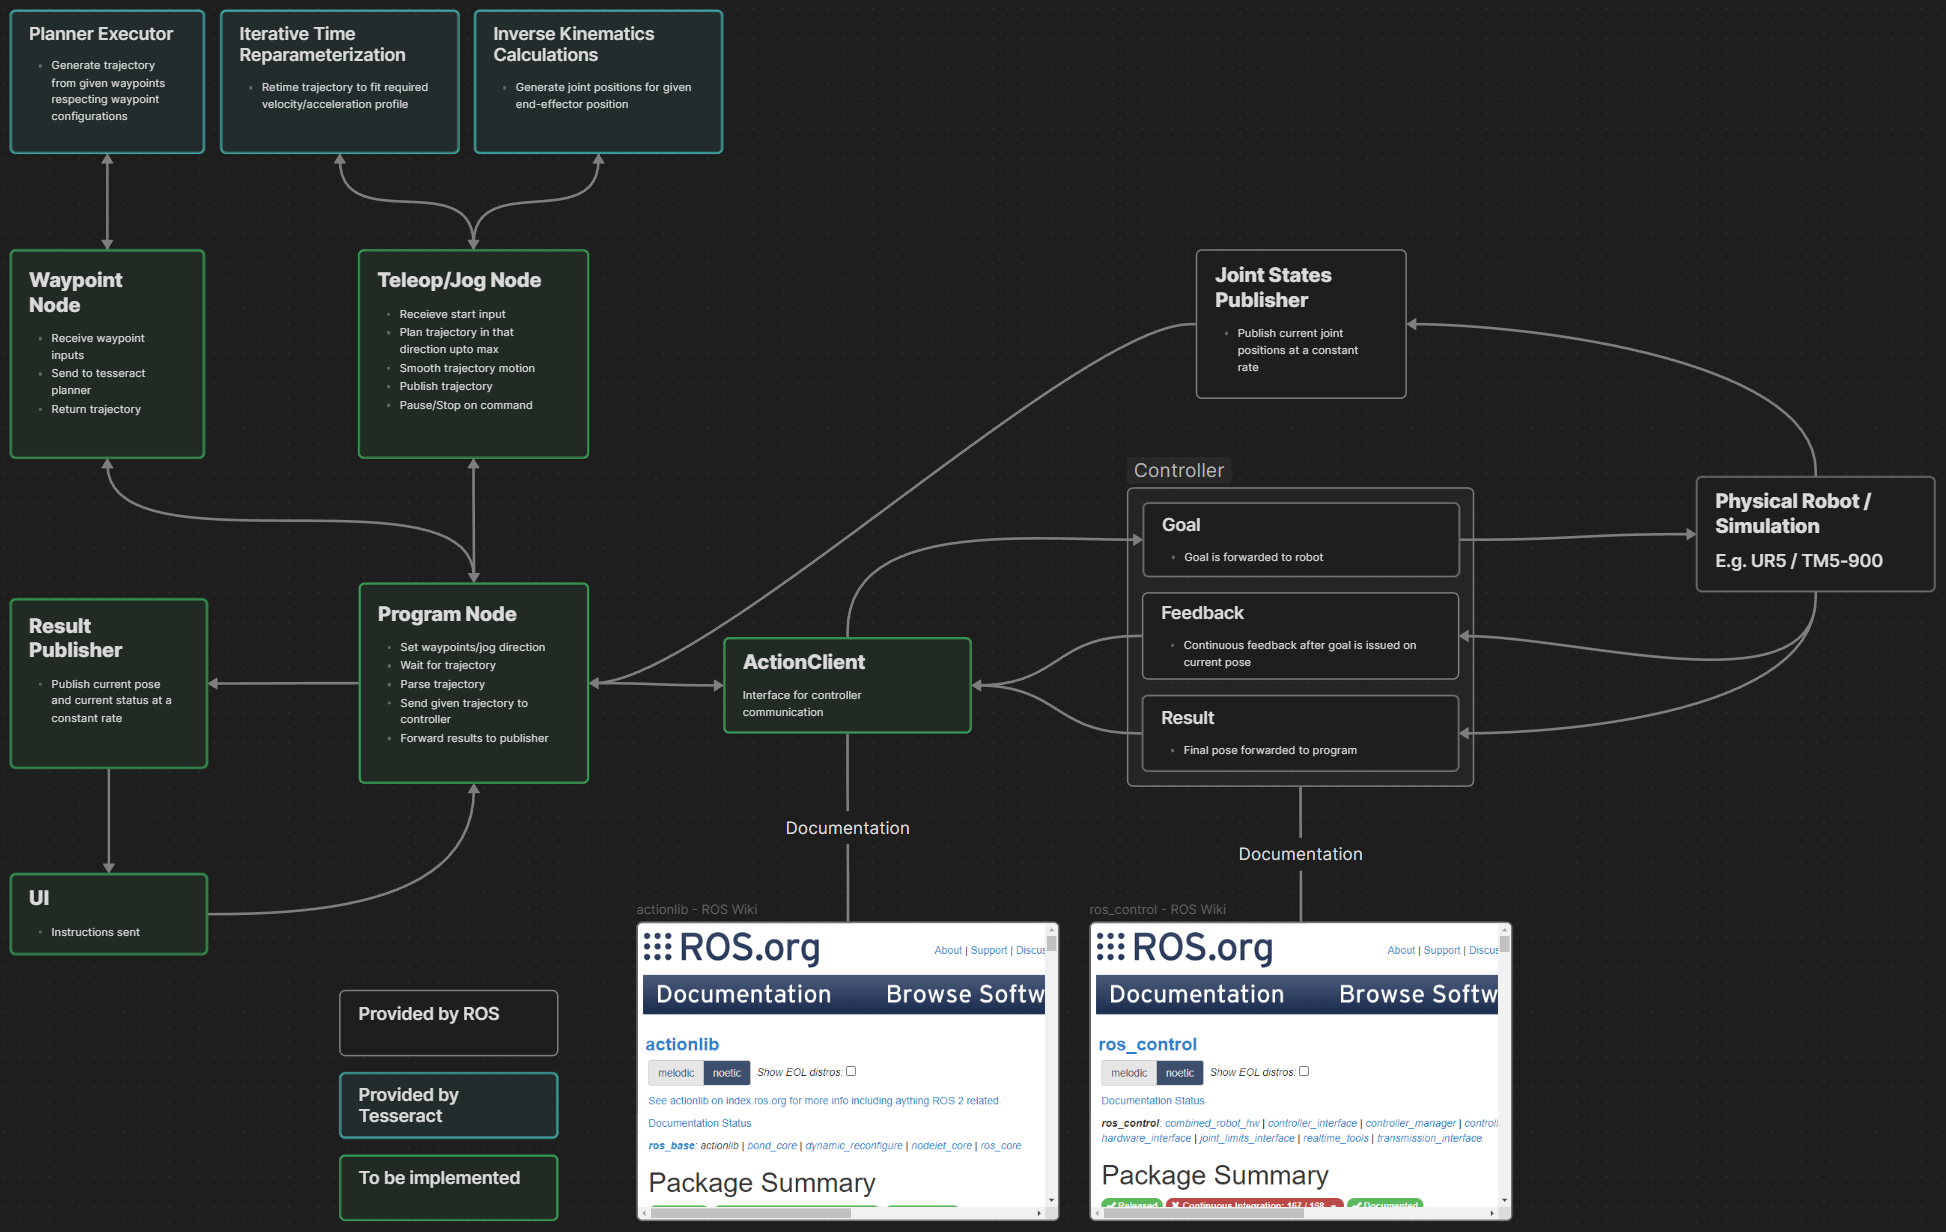
\includegraphics[width=.8\linewidth]{robot-diagram}
    \caption{A high-level diagram showing interactions between ROS, Tesseract, and the manipulation
        library. It also details how the trajectory controller middleware works, with the goal
        endpoint forwarded to the robot, and feedback states returned to the
        application.\label{fig:robot-diagram}}
\end{figure}

By documenting my actions, I began to better appreciate the more well-documented code I've seen -
something I had previously taken for granted. Many hours of frustration and debugging could have
been mitigated had basic documentation been available. Following this, efforts have been made to
actively document all aspects of my work, including personal projects.

\subsection{Implementation}

As Tesseract is only a framework for motion planning, planning algorithms still needed to be
selected for usage. My colleagues and I evaluated several algorithm implementations, primary ones
being TrajOpt, \acro{ompl}, and Descartes. For each, we outlined the benefits and drawbacks of each
approach along with an evaluation of practical performance.

For instance, TrajOpt was notable in its ability to not only produce reliable trajectories under
complex constraints, but also in its ability to have initial conditions be seeded by other planners,
providing more robust solutions. Usage of TrajOpt also allowed for both joint space and Cartesian
space planning, as specific constraints could be supplied to the algorithm depending on the type of
motion required. However, TrajOpt was significantly slower to execute than other planners like
\acro{ompl}. It should be noted that Tesseract supported the ability to change planners at runtime,
allowing for adaptability if a certain task was more suited towards another planner.

Implementing joint and Cartesian teleoperation in the library brought unexpected challenges. While
the implementation of joint space teleoperation was relatively simple (adjusting the position value
of a single joint in response to user input), it was quite difficult to perform real-time Cartesian
teleoperation as moving along a line/axis involves the movement of all joints in a non-intuitive
manner.

My approach to this problem was to use \acro{ik} -- \acrodesc{ik} -- to formulate a trajectory along
a given axis. Additionally, after searching through the Tesseract library code, I was able to apply
Tesseract's post-processing abilities onto my trajectory, ensuring a collision free trajectory and
allowing joint velocity values to be generated alongside the \acro{ik} positions. These were tested
vigorously by myself and others in simulation software (Gazebo) as well as on a physical robot arm,
interfacing with a small terminal program I wrote that converted key presses to robotic movement
(Fig.~\ref{fig:robot-terminal}).

\begin{figure}
    \centering
    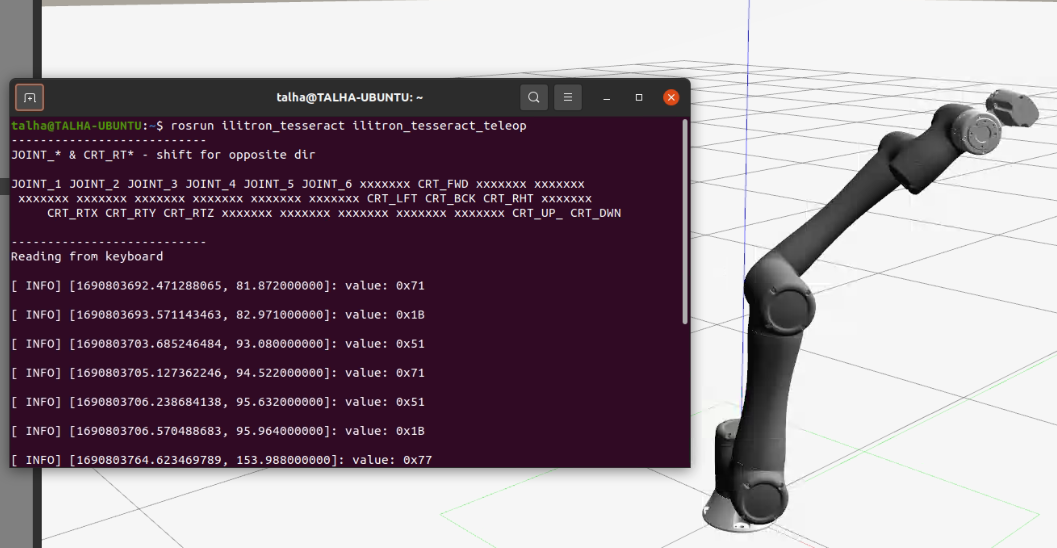
\includegraphics[width=\linewidth]{robot-tui}
    \caption{A terminal application for teleoperation, acting on a simulated robot. Key inputs would
        be translated to library calls, resulting in arm motion.\label{fig:robot-terminal}}
\end{figure}

During this project I realized how imperative testing is in these safety-critical situations, as
numerous fail-safes -- some of which I triggered -- were put in place to prevent unexpected or dangerous
movement when running my teleoperation code on the physical arm. This ranged from software measures
to avoid self-collision and halt movement before irregular velocities or positions were reached, as
well as physical measures such as having more than one person observing the robot. Coming from a
background of no robotics nor embedded software development, this was an aspect of development I had
never encountered before and taught me how different testing can be.

\section{Other projects}

The following subsections are a non-comprehensive overview of smaller projects worked on between the
larger projects detailed above.

\subsection{Task Management Web Application}
\label{sec:task-app}

During the placement, a need for a task management and monitoring tool arose to coordinate projects
between colleagues. An off-the-shelf \acro{saas} solution for project management would easily fulfil
this need, however an in-house solution was desired to facilitate any further requirements that may
arise. A primary need was the ability for employees to self-report the estimated progress of their
tasks, as well as for managers to evaluate the progress of employees. I was asked to develop a proof
of concept web application that could be deployed on premises for these requirements.

The technologies I picked for this project was React (a web framework) written with TypeScript (a
typed superset of JavaScript), and a MySQL relational database. These were primarily selected due to
my familiarity with this stack allowing me to quickly iterate on the prototype application. Styling
was handled by the Bootstrap, a CSS framework providing styled components, to allow for more focus
on functionality with the intention of replacing with custom styling later. This was then placed
behind a single sign-on page utilizing company authentication.

\acro{rbac} was used to provision different features of the app to different groups of people.
Regular employees were only able to view and update tasks assigned to them, and admins were given
full view and edit access to the whole organization. Implementing \acro{rbac} allowed for additional
roles to be easily implemented, such as managers who were given the ability to create and modify
tasks only for people in their respective teams.

Prototypes were deployed to teams within the company, from which I received constant feedback
regarding requirements, changes, as well as what worked well, all of which aided in refining the
application. While development of these features were straightforward, it was particularly
challenging to prioritise changes that at times even conflicted with one another, requiring the need
to create diagrams and mock-ups for clarifying details.

One notable non-trivial change that was requested was the ability to create groups that could
contain subgroups and tasks (Fig.~\ref{fig:website-overview}), akin to directories containing
subdirectories and files in an operating system's hierarchical file system. This involved modifying
the database schema and queries to support recursive relationships. An aspect that was initially
overlooked was the amount of time a query would take to recurse through the task tree using a
depth-first search, causing the user interface to feel slow and unresponsive when looking through
task groups.

To mitigate against this, groups were appended with metadata to reduce the search depth
in queries, such as adding a \enquote{path} of groups to a task and storing the aggregate progress
of a group in the database rather than computing at runtime. This time-memory trade-off allowed for
significantly faster navigation between groups without the time penalty of querying down the task
tree.

\begin{figure}
    \centering
    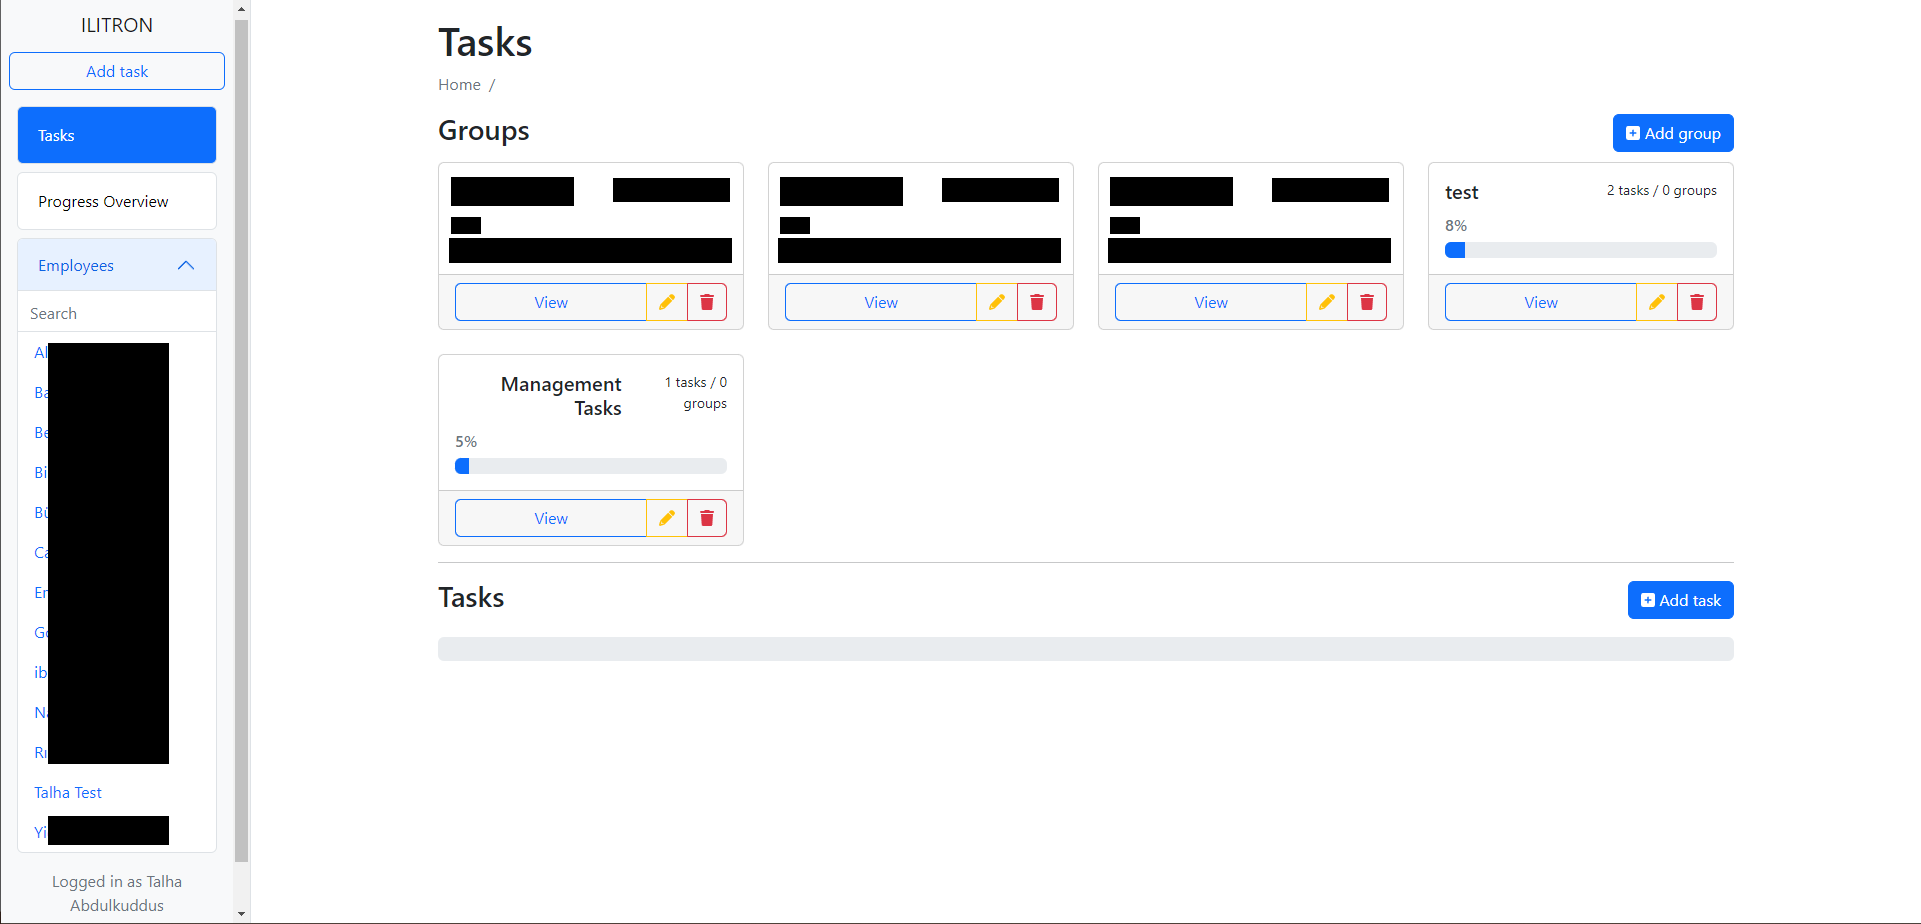
\includegraphics[width=\textwidth]{website-overview}
    \caption{Overview of all top-level groups and tasks, each including its aggregate
        progress.\label{fig:website-overview}}
\end{figure}

This project gave me an insight into the full software development process, from eliciting
requirements and features to deploying to users. It educated me on the skills necessary to decipher
user needs and iterating on an application that is actively in deployment.

\subsection{EU Horizon Europe Proposal}
\label{sec:eu-proposal}

Horizon Europe is the EU's research funding programme which \enquote{facilitates collaboration and
    strengthens the impact of research and innovation in developing, supporting and implementing EU
    policies while tackling global challenges} \autocite{horizoneurope}. Projects proposals
submitted to Horizon Europe are expected to contribute to a specific \enquote{call}, which is a
specific set of outcomes the EU expects projects to meet.

ILITRON intended to collaborate with other organizations and universities, proposing a specific
project under the call: \enquote{Novel paradigms and approaches towards AI-driven autonomous
    robots}. As I had some experience with RL in robotics, direct robot control software, as well as
being a native English speaker, I was asked to participate in writing up the project proposal for
this call with my colleagues.

A typical Horizon Europe proposal is split into three sections:

\begin{itemize}
    \item Excellence, detailing objectives, how the project pushes the state-of-the-art, and the
          project methodology;
    \item Impact, detailing how the project contributes to the call's outcomes with societal
          impact, as well as project's dissemination strategies;
    \item and a work plan detailing the responsibilities each organization will take on for the
          project.
\end{itemize}

My responsibility was collecting information to introduce the project and it's objectives in the
Excellence section, and assisting in writing the Impact section of the proposal.

To ensure the content of the proposal remained relevant to the call provided by the EU programme, I
was asked to provide a presentation to colleagues on how the proposal should be written within each
section, according to guidelines provided by the programme. I also produced an accompanying document
outlining these points for people to refer back to during their work. Throughout the writing stage I
analysed the proposal, providing advise when asked by colleagues, and suggesting changes in wording
and structure.

For the Excellence section, I collaborated with others in reducing the full methodology to its novel
ideas and implementations, from which I authored the introduction to the document. It was critical
that the objectives in this section could be analysed quantitatively, in order to demonstrate
objective progress being made. Key objectives were discussed with the team, such as the resultant
deep \acro{rl} agent expected to be produced, and the \acro{kpis} for each objective to be
considered fulfilled, such as the percentage accuracy of the deployed \acro{rl} agent.

The Impact section involved analysing the proposal to inform how it is in line with the given call,
as well as identifying potential barriers to implementation. This turns out to be of utmost
importance when implementing an \acro{ai}-driven robot, as many issues could potentially arise
during development (such as lack of training data, non-standardized working environments,
insufficient mechanical tolerances, etc.). These issues were not restricted to being technical, as
they needed to comprehensively cover all potential impacts including market and regulatory barriers,
such as ethical considerations for our use of \acro{ai}\@. These potential issues were discussed
between my colleagues and I, and a list of mitigation measures were introduced to reduce the effect
of these problems, subsequently strengthening the overall proposal.

Following the submission of the proposal, I was asked to help create a company-wide presentation
along with a few of my colleagues about the experience of authoring each section of the proposal.
The purpose of this was to inform others in the company on the process of participating in these
government funded programmes, while also making those who participated in the proposal (my
colleagues and I) reflect on the project as a whole.

This was one task I was not comfortable on performing, especially considering all other parts of the
presentation excluding mine were to be presented in Turkish. However, I was encouraged by several
people to participate in presenting regardless, with a colleague willing to translate to others if
it was necessary. Despite my earlier preconceptions about presenting in a different language to
others, the presentation went smoothly and helped me gain confidence in presenting to others,
including foreign audiences.

Working on this project was a unique experience as it followed very closely to the early stages of
waterfall software development, a sequential approach to the software development lifecycle, whilst
adhering to a specific framework of rules and regulations set by the EU\@. This project also
provided me the opportunity to work with colleagues across the company, some who I had not worked
with before.
